
\section{\tc Implementation Details}
\label{sec:impl}

In our implementation of TC, we use Ethereum smart contracts and an SGX enclave to provide trusted computing environments.
The details of resource management within Ethereum present new challenges as they open TC to new attacks.

During the creation and fulfillment of any request, there are two untrusted parties:
the requesting user and the TC relay and network (which we view as a single adversary).
The protocol discussed in Section \ethan{ref no-gas} guarantees authenticity of data for an honest requester even in the face of a malicious relay.
However, the TC system has no vulnerable resources and requests are separated from each other preventing a malicious user from causing harm.
In Ethereum, executing computation is not free.
This means that TC needs to maintain enough money to deliver datagrams which means users must pay a fee to reimburse costs.
The fee raises the concern that a compromised relay may be able to prevent delivery of a datagram and cost an honest requester money for no gain.

While designing the implementation, we consider three cases:
\begin{itemize}
  \item {\it Honest requester and relay.}
    The requester must receive a valid authenticated response from TC.

  \item {\it Malicious requester and honest relay.}
    TC must still be able to respond correctly to requests from other (honest) users.
    To do this, we must prevent a malicious user from interfering directly with other requests (which we cover in our payment-free protocol in Section \ethan{ref no-gas})
    or exhausting the financial resources of TC.

  \item {\it Honest requester and malicious relay.}
    The requester cannot receive invalid data that looks valid (which we is also guaranteed by our payment-free protocol)
    and the requester must lose a bounded amount of money.
\end{itemize}
We formalize these properties in Section \ethan{refer} and prove that our protocol provides these guarantees.
We intentionally ignore the case where both the requester and the relay are dishonest.
If the requester is dishonest we need to not protect their request, and if the relay is dishonest we cannot protect the TC system.


\subsection{Handling Fees in Ethereum}
\label{sec:gas-protocol}




As we described in Section~\ref{sec:contracts-and-gas}, Ethereum employs \emph{gas}, a fee mechanism, to mitigate DoS attacks.
In order to sustainably operate \tc on Ethereum, we develop a novel two-currency resource management system which allows
\tc to make gas payments up front while preventing a malicious requester from exhausting \tc's resources.


\paragraph{Execution model and notation.}

%We assume the blockchain contract adopts the following execution model which closely resembles that of Ethereum described in Section \ethan{refer}.
%
%\begin{itemize}[leftmargin=1.5em]
%  \item {\it Providing gas.}
%    When a transaction is submitted, it invokes an entry point in the contract and provides a gas amount.
%
%  \item {\it Extra gas.}
%    If the provided gas exceeds the gas necessary to process the transaction, all excess gas is refunded as part of the transaction.
%
%  \item {\it Gas exhaustion.}
%    Consider each entry point a function call.
%    If a function calls another function, the parent may limit the gas available to the child to a value no higher than the gas available to the parent.
%    When a function cannot complete execution within its gas limit,
%    that function execution is aborted and all state is reverted to immediately prior to that call.
%    Note that if the initial entry point runs out of gas, the entire transaction is aborted.
%
%\end{itemize}

We take Ethereum's gas model ask described in Section~\ref{sec:contracts-and-gas}.
We use the notation $\gas$ to denote gas and $\fee$ to denote non-gas currency.
In both cases \$ is a type annotation and the letter denotes the numerical amount.
For simplicity, our notation assumes that gas and normal currency adopt the same units (allowing us to perform arithmetic without conversion).
We use the following identifiers to denote currency and gas amounts.
%
\begin{center}
\begin{tabular}{m{0.08\columnwidth}m{0.85\columnwidth}}
  \hline
  $\fee$
  & Currency a requester deposits to refund \tcs's gas expenditure to deliver a datagram \\
  \hline
  $\gasdeliver$ $\gasrequest$
  & {\tt GASLIMIT} when invoking {\bf Deliver} and {\bf Request}, respectively \\
  \hline
  $\gascallback$
  & {\tt GASLIMIT} for $\dgcallback$ while executing {\bf Deliver}, set to the max value that can be reimbursed \\
  \hline
  $\constgasmin$
  & Gas required for {\bf Deliver} excluding $\dgcallback$ \\
  \hline
  $\constgasmax$
  & Maximum gas \tc can spent to invoke {\bf Deliver} \\
  \hline
\end{tabular}
\end{center}
%
Note that $\constgasmin$ and $\constgasmax$ are system constants,
$\fee$ is chosen by the requester (and may be malicious if the requester is dishonest),
and $\gasdeliver$ is chosen by the \tc~\encname when calling {\bf Deliver}.
Though $\gasrequest$ is set by the requester, we need not worry about the value.
If it is too small, Ethereum will abort the transaction and there will not be a request.


%\begin{figure}
%\centering
%\begin{tikzpicture}
%  [local-entity/.style={entity,minimum height=3.5em,text width=8em}]
%  \node[local-entity,trusted] (ctc) {};
%  \node[local-entity,draw=none,anchor=north] (ctc-inner) at (ctc.north) {TC Contract\\$\tcont$};
%  \node[local-entity,trusted,right=6em of ctc,text width=5em] (enc) {Enclave};
%  \node[local-entity,fill=white,below=3.5em of ctc] (cu) {User Contract\\$\reqcont$};
%  \node[local-entity,fill=red!30,below=2.5em of cu] (user) {User};
%
%  \path[-stealth,color=red,ultra thick] (user) edge [transform canvas={xshift=-3.5em}] ([yshift=0.75em]cu.south);
%  \path[color=red,thick] (cu.south) edge [right,transform canvas={xshift=-3.5em}] node [text=black,text width=4em,align=center,yshift=1.75em] {\footnotesize Insufficient\\[-0.25em]gas aborts\\[-0.2em]with no\\[-0.5em]effect} (ctc.south);
%  \node[draw=red,cross out,minimum size=1ex,thick] () at ([xshift=-3.5em]ctc.south) {};
%
%  \draw[-stealth,color=green!50!black,line width=0.8ex] ([yshift=-0.25em]enc.west) -- ([xshift=-1.2em,yshift=-0.25em]ctc.east);
%  \draw[-stealth,color=green!50!black,line width=0.5ex] ([yshift=-0.25em]enc.west) -| ([xshift=3em,yshift=-0.9em]cu.north);
%  \draw[color=green!50!black,thick,dashed]  ([xshift=3.75em]cu.north) |- ([yshift=-1.25em]ctc.east);
%  \path[-stealth,color=green!50!black,ultra thick,dashed]  ([yshift=-1.25em]ctc.east) edge [below] node [text=black,text width=4em,align=center,xshift=-0.4em] {\footnotesize Extra gas\\[-0.4em]refunded} ([xshift=0.8em,yshift=-1.25em]enc.west);
%
%  \begin{pgfonlayer}{background}
%    \node[bg-box,
%          blockchain-color,
%          fit={($(ctc.north west)+(-0.5em,0.5em)$)($(cu.south east)+(0.5em,-0.5em)$)},
%          label=above:{\bf Blockchain}] () {};
%    \node[bg-box,
%          tc-server-color,
%          fit={($(enc.north east)+(0.5em,0.5em)$)($(enc.south west)+(-0.5em,-0.5em)$)},
%          label=above:{\bf TC Server}] () {};
%  \end{pgfonlayer}
%\end{tikzpicture}
%\caption{{\bf Gas Payment in Ethereum}}
%\label{fig:gas-model}
%\end{figure}



\begin{figure}
\begin{tabularx}{\linewidth}{|@{\hspace{3pt}}r@{\hspace{1ex}}X@{\hspace{3pt}}|}
  \hline

  \multicolumn{2}{|c|}{{\bf \tcs blockchain contract \tcont with fees}} \\[1ex]
  {\bf Request:} & On recv $({\sf params}, {\sf callback}, \fee, \gasrequest)$ from some $\reqcont$: \\
                 & Assert $\constgasmin \leq \fee \leq \constgasmax$ \\
                 & $\dgid := \text{Counter}$; \ \ $\text{Counter} := \text{Counter} + 1$ \\
                 & Store $(\dgid, \dgform, \dgcallback, \fee)$ \\[-0.8em]
                 & {\it \sgray{//~$\fee$ held by contract}} \\

  {\bf Deliver:} & On recv $(\dgid, \dgform, \dgm, \gasdeliver)$ from $\tcadd$: \\
                 & Retrieve stored $(\dgid, \dgform', \dgcallback, \fee)$ \\
                 & \quad \sgray{\it //~abort if not found} \\
                 & Assert $\dgform = \dgform'$ \\
                 & Assert $\fee \leq \gasdeliver$ \\
                 & Send $\fee$ to \tcadd \\
                 & Set $\gascallback := \fee - \constgasmin$ \\
                 & Call $\dgcallback(\dgm)$ with $\gascallback$ max gas \\
  \hline
\end{tabularx}
\caption{
Town Crier contract \tcont reflecting fees.
The last argument of each entry point is the {\tt GASLIMIT} provided.
An honest requester sets $\fee$ to be the gas amount
required to execute the {\bf Deliver} entry point including $\dgcallback$.
Town Crier sets $\gasdeliver := \constgasmax$, but lowers the gas limit for $\dgcallback$ ensure that no more than $\fee$ is spent.
}
\label{tbl:gas-tc-contract}
\end{figure}

\begin{figure}[!h]
\begin{boxedminipage}{\columnwidth}
\centering
{\bf Program for \tcs~\encname ($\enclaveprog$)} \\[1ex]
\begin{tabular}{l}
  {\bf Initialize}: Same as Figure \ethan{refer} \\[3pt]

  {\bf Resume:} On recv $(\resumecall, (\dgid, \dgform))$ \\
  \quad Same as before except the last two statements: \\
  \quad $\sigma := \Sigma.{\sf Sign}({\skTC}, (\dgid, \dgform, \dgm, \constgasmax))$ \\
  \quad Output $((\dgid, \dgform, \dgm, \constgasmax), \sigma)$ \\
\end{tabular}
\end{boxedminipage}
\caption{The \tcs~\encname \engine.}
\label{fig:engineprot}
\end{figure}

\begin{figure}
\centering
\begin{tikzpicture}
  [contract/.style={entity,minimum height=3.5em,text width=7.5em},
   wallet/.style={entity,minimum height=3.5em,text width=5em},
   type-box-color/.style={fill=black!10},
   blocked-out-label/.style={text=black,type-box-color,text height=0.6em}]
  \node[wallet,fill=white] (user) {User ${\cal P}_U$};
  \node[contract,fill=white,right=6em of user] (cu) {User Contract\\$\reqcont$};
  \node[wallet,trusted,below=5em of user] (tc-wallet) {$\tcadd$};
  \node[contract,trusted,right=6em of tc-wallet] (ctc) {TC Contract\\$\tcont$};
  \node[color=maroon,draw,anchor=south east] (fee) at ([xshift=-0.25em,yshift=0.25em]ctc.south east) {\small $\fee$};

  \draw[color=gold,rounded corners,opacity=0.25,line width=1ex] ([yshift=1.25em]user.east) -| ([xshift=3.25em]cu.south);
  \path[-stealth,color=gold,line width=1.15ex] (user) edge [transform canvas={yshift=1.25em}] (cu);
  \path[-stealth,color=gold,line width=1ex] (cu) edge [transform canvas={xshift=3.25em}] (ctc);
  \path[-stealth,color=maroon,line width=0.4ex] (cu.south) edge [left,transform canvas={xshift=3.25em}] node [blocked-out-label,xshift=1em,yshift=1.2em] {\small \smash{$(\gasrequest, \fee)$}} ([yshift=-1.5em]ctc.north);
  \node[anchor=north,xshift=1em,yshift=-0.75em] () at (cu.south) {\small \bf \underline{\smash{Request}}};

  \path[-stealth,color=gold,line width=1ex] (tc-wallet.east) edge [above,transform canvas={yshift=0.4em}] node () {\small $\gasdeliver$} (ctc.west);
  \draw[color=gold,rounded corners,opacity=0.25,line width=0.3ex] ([yshift=0.4em]tc-wallet.east) -| ([xshift=-3em]ctc.north);
  \path[-stealth,color=gold,line width=0.3ex] (ctc.north) edge [right,transform canvas={xshift=-3em}] node [yshift=-1.25em] {\small \smash{$\gascallback$}} (cu.south);
  \path[color=maroon,opacity=0.25,line width=0.4ex] (tc-wallet-|fee.west) edge [transform canvas={yshift=-1.25em}] (tc-wallet.east);
  \path[-stealth,color=maroon,line width=0.4ex] (ctc.west) edge [transform canvas={yshift=-1.25em}] node [blockchain-color,xshift=0.4em] {\small $\fee$} ([xshift=-0.8em]tc-wallet.east);
%  \path[-stealth,color=gold,ultra thick,dashed] (ctc.west) edge [below,transform canvas={yshift=-1em}] node [text=black,xshift=0.4em] {\small $\gasdeliver - \fee$} ([xshift=-0.8em]tc-wallet.east);

  \path[] (tc-wallet.north east) edge [draw=none,above] node [yshift=0.75em] {\small \bf \underline{Deliver}} (ctc.north west);

  \begin{pgfonlayer}{background}
    \node[bg-box,
          blockchain-color,
          fit={($(ctc.south east)+(1em,-1em)$)($(user.north west)+(-1em,2em)$)},
          label=above:{\bf Blockchain}] () {};
    \node[bg-box,
          type-box-color,
          fit={($(ctc.south east)+(0.5em,-0.5em)$)($(cu.north west)+(-0.5em,0.5em)$)},
          label=above:{\bf Contracts}] () {};
    \node[bg-box,
          type-box-color,
          fit={($(tc-wallet.south east)+(0.5em,-0.5em)$)($(user.north west)+(-0.5em,0.5em)$)},
          label=above:{\bf Wallets}] () {};
  \end{pgfonlayer}
\end{tikzpicture}
\caption{{\bf Blockchain Money Flow within Town Crier.}
Red arrows denote flow of money and brown arrows denote gas provided for function execution.
The thickness of the line indicates the quantity of the resource.
The $\gascallback$ is thin because that value is limited by {\bf Deliver} to $\fee - \constgasmin$.
}
\label{fig:money-flow}
\end{figure}



\paragraph{Town Crier protocol with transaction fees.}
Our basic Town Crier system implements a policy where the requester pays for all gas needed and Town Crier effectively pays nothing.
We now describe how this can be realized by modifying the fee-free protocol described in Section \ethan{refer}.

\begin{itemize}[leftmargin=1.5em]
  \item {\it Initialization.}
    We assume that Town Crier deposits at least $\constgasmax$ into the wallet $\tcadd$.

  \item {\it \tcs blockchain contract.}
    Figure \ref{tbl:gas-tc-contract} describes the \tcs blockchain contract reflecting fees.
    Since $\tcadd$ must invoke {\bf Deliver}, \tc will pays the gas cost.
    It sets the {\tt GASLIMIT} $\gasdeliver := \constgasmax$.
    To ensure that the gas spent will not exceed the reimbursement available ($\fee$),
    \tcont sets the {\tt GASLIMIT} $\gascallback$ for the sub-call to $\dgcallback$ to the reimbursement remaining: $\fee - \constgasmin$.

  \item {\it Town Crier Relay.}
    The relay behavior does not change with the presence of fees.
    It still monitors the blockchain and whenever the contract \tcont stores a new request $(\dgid, \dgform, \_, \_, \_)$,
    it invokes $\enclaveprog$ with $\resumecall(\dgid, \dgform)$.

  \item {\it Town Crier enclave.}
    We make the following small modification to the fee-free protocol.
    Instead of signing the tuple $(\dgid, \dgform, \dgm)$ at the end of its execution,
    the enclave now signs the tuple $(\dgid, \dgform, \dgm, \gasdeliver)$ where $\gasdeliver = \constgasmax$.

  \item {\it Requester.}
    An honest requester behaves the same was as in Figure \ethan{refer} except for setting a {\tt GASLIMIT} of $\gasrequest$ and sending $\fee$ money with each request.
    It sets $\gasrequest$ to be at least the cost of executing the {\bf Request} entry point
    and $\fee$ to be the cost of executing the {\bf Deliver} entry point (including executing the user-defined $\dgcallback$ function).
\end{itemize}

We prove in Section~\ref{sec:analysis} that this protocol ensures authenticity of the datagram, that \tc cannot lose money when the \medname is honest,
and that an honest requester's loss is bounded even against a malicious \tc.






\subsection{TC Contract}

We implemente \tcont with fees as described in Section~\ref{sec:gas-protocol} in Solidity,
a high-level language with JavaScript-like syntax which compiles to Ethereum Virtual Machine bytecode---the language Ethereum contracts use.

In order to handle the most general type of requests---including encrypted parameters---the \tcont implementation requires two parameter fields.
The first is a single byte specifying what type of request is being made (e.g. stock price or flight status).
The second is a byte array of user-specified size.
This byte array will be parsed and interpreted inside the enclave when it fulfills the request, but is treated as an opaque byte array by \tcont.

As we discuss in Section \ethan{ref authenticity}, \tcont must store the parameters and \tc must pass them back in {\bf Deliver} to ensure that the request has not been modified.
In order to reduce the verification costs for requests with long parameter arrays, we instead store and verify a hash of the parameters.
In particular, we store the SHA3-256 hash of the concatenation of the request type byte and the byte array.
The relay scrapes the actual parameters and passes them into the enclave.
When calling {\bf Deliver}, \enclaveprog computes the same hash and passes that back for validation.
This allows us to continue validating long requests at low cost.



\subsection{TC Server}
% programming model
% ecall and ocall

\subsubsection{Overview of SGX-enabled applications}

Using the recently released Intel SGX SDK~\cite{sgxsdk}, we implmented the \tc
Server as an SGX-enabled application in C++. The programming model employed by
the SDK is that the major body of an SGX-enabled application remains an
ordinary user-space application, while an relatively small piece of security-sensitive code
is teased out and runs in an isolated environment, namely in an SGX enclave.

The enclave part of an SGX-enabled application can be
viewed as a shared library exposing APIs, referred to as \emph{ecalls} by~\cite{sgxsdk},
to be invoked by the untrusted application. However, unlike a share library,  
once ecalls are invoked, the control is transferred to the 
enclave code until it finishes or some special event happens~\cite{sgxmanual}.
As we assume SGX provides a perfect isolation, the untrusted application can not
observe or alter the execution of ecalls.

In addition, the SGX SDK implements a mechanism called \emph{ocall} with which enclave
programs can invoke functions defined outside of the enclave. In essence,
calling an ocall causes the enclave program first to exit the enclave. Once the
ocall is fulfilled, execution is transferred back to the calling enclave. 
Although it is permissible to make arbitrary ocalls, special caution must be 
as ocalls are fulfilled in the untrusted world.
The ocall interface between \encname and \medname is carefully designed such that the 
the \medname can not subvert the security of \tc.

In the context of TC Server, the enclave part implements Figure. \fan{ref to
prog}, which encompasses the implementation of a TLS layer, a partial HTTP
layer, a set of algorithms that extract information from web pages, and a
request handler that can parse and generate Ethereum transactions and sign it
properly with \skTC.  The untrusted part of TC Server implements Figure \fan{ref
to prog}, which roughly encompasses of two parts: (1) an access point to various
OS services, (2) an interface with Ethereum blockchain and (3) an interface with
clients. Figure \ref{fig:tcserver_impl} summarizes these components and their
interaction.

\begin{figure}[h]
    \centering
    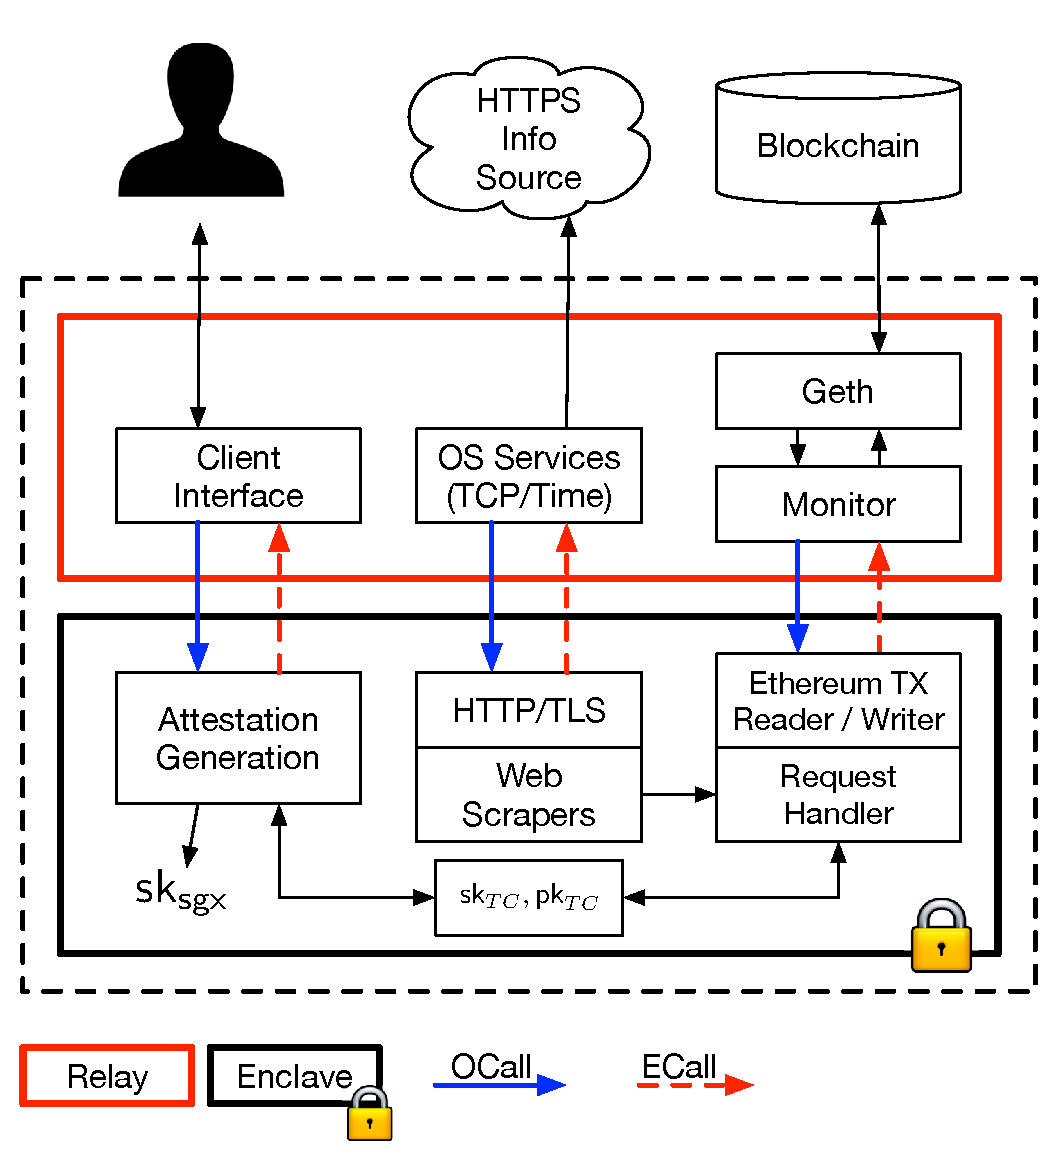
\includegraphics[width=0.4\textwidth]{figures/impl}
    \caption{Detailed Architecture of TC Server}
    \label{fig:tcserver_impl}
\end{figure}

\subsubsection{The \medname}

\paragraph{Attestation Server.} As described in Section \ref{sec:architecture},
a client starts using \tc by requesting and verifying an attestation.  The
Attestation Server (AttServer) is the interface for doing this.  The AttServer
listens for requests and calls into the Attestation Generation logic in the
enclave (by making an ecall) to get an attestation, along with an Unix timestamp
signed by \pkTC, and forward both to the requesting client.  The EPID group
signature can verified by accessing Intel Attestation Service (IAS)~\cite{}. 

\paragraph{OS Services.} The \encname relies on \medname for networking and
time provided by the OS. We implemented wrapper functions for these OS services 
that can be invoked by the \encname as ocalls.

\paragraph{Blockchain Interface.} The \medname is responsible to watch the
blockchain for incoming requests and insert transactions to the blockchain to
deliver datagrams. To interact with the Ethereum blockchain, we incorporated an
official Ethereum client (geth~\cite{geth} in particular) into the \medname.
Geth client can be configured to setup a JSON RPC server through which the
Monitor can communicate with the blockchain indirectly by sending RPC calls to
geth. For example, to insert a signed transaction, the Monitor can simply call
\texttt{eth\_sendRawTransaction} with the bytes array of the serialized
transaction, and geth do the rest of the work. Looping an Ethereum
client into \medname saves us the cost of reinventing the wheel. 
Note that the signing of transactions is done within the enclave, as the key
\pkTC only accessible to the enclave program.

\subsubsection{The \encname}

\paragraph{HTTPS in the \encname.} 
The \encname needs the TLS layer to talk with remote HTTPS web servers.  We
ported a TLS library (mbedTLS) into the SGX environment so it can be used within
the enclave.  To verify the certificates presented by remote servers, a
collection of trusted root CAs are manually selected \xxx[Fan]{what's the best
practice? Maybe we can choose the same root CAs as Chrome or Firefox?} and their
certificates are hardcoded in the enclave program. A certificate is verified
only if it is finally issued by one of the trusted root CA.

\paragraph{Web Scrapers.} Extracting useful information from a given website is
implemented in a ad-hoc manner. For the purpose of demonstration, we implemented
three web scrapers as examples. \xxx[Fan]{Elaborate}.

\paragraph{Request Handler} Request handler has two jobs: 1) to parse the
request which is serialized in the format specified by Ethereum ABI, decrypt it if encrypted under
\pkTC, and dispatch it to the right scraper; 2) to generate a Ethereum
transaction, sign it with \pkTC and serialize it properly so that it can be
inserted to the blockchain. In essence, we implemented the Ethereum ABI and RLP which
specifies the serialization of arguments and transactions respectively.
In addition, the signature algorithm used in signing Ethereum transactions is
ECDSA on the curve Secp256k1. SHA3 is used to generate message digests.

\paragraph{Attestation Generation} The same with Attestation Server.\xxx[Fan]{Elaborate.}
\paragraph{Key Management} \xxx[Fan]{TBD.}


